% Author: Seongjin Lee 
% Hanyang University, Seoul, Korea 
% esos.hanyang.ac.kr 
% 2016-09-20
% note: some slides are adopted from  \url{www.cs.stevens.edu/~jschauma/631A/}
% https://github.com/resourceful/lecture_sysprog/

\documentclass[newPxFont,sthlmFooter,nooffset]{beamer}
\usepackage{kotex}
%\usetheme{sthlm}
\usepackage{../beamer_template/beamerthemesthlm}
\hypersetup{pdfauthor={Seongjin Lee (insight@hanyang.ac.kr)},
            pdfsubject={Lecture Note: System Programming},
            pdfkeywords={Lecture Note, System Programming, class, undergraduate},
            pdfmoddate={D: \pdfdate},
            pdfcreator={Seongjin Lee}}

%\setbeamertemplate{footline}[text line]{%
%    \parbox{\linewidth}{\vspace*{-8pt} \insertsectionhead  \hfill\insertshortauthor\hfill\insertpagenumber}}
%\setbeamertemplate{navigation symbols}{}




\title{System Programming}
\subtitle{Week 7: Process Relationships}
\author[SJL]{Seongjin Lee}
\institute{\href{mailto:insight@hanyang.ac.kr}{insight@hanyang.ac.kr}\\\url{http://esos.hanyang.ac.kr}\\Esos Lab. Hanyang University}
\date{2016-10-19} 

\begin{document}



\frame[plain]{\titlepage} 

\frame[t]{\frametitle{Table of contents}\tableofcontents} 


%---------------------------------------------------------



\begin{frame}[t]
  \frametitle{introduction}
This chapter covers following items
  \begin{itemize}
  \item Terminal Logins
  \item Sessions
  \item Controlling Terminal
  \item Job Control
  \end{itemize}

\end{frame}



\section{Terminal Logins}

\begin{frame}[t]
  \frametitle{Terminal}
  \begin{figure}[h]
    \centering
    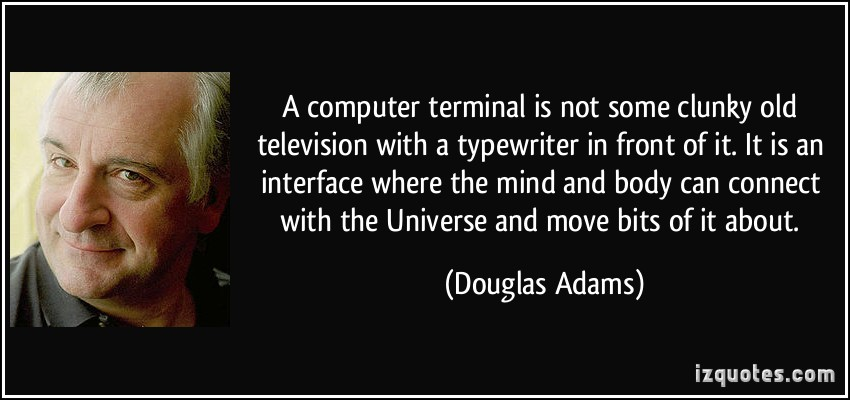
\includegraphics[width=0.8\linewidth]{figure/quote-a-computer-terminal-is-not-some-clunky-old-television-with-a-typewriter-in-front-of-it-it-is-an-douglas-adams-296711.jpg}
    \caption{Douglas Noel Adams was an English author, scriptwriter, essayist, humorist, satirist and dramatist, best known as the author of The Hitchhiker's Guide to the Galaxy'' 1978}
  \end{figure}
\end{frame}


\begin{frame}[fragile,t]
  \frametitle{Terminal Logins}
In early \textsc{Unix} systems
\begin{itemize}
\item <1-> Users logged in using dumb terminals that were connected to the host with hard-wired connections
\item <2-> The terminals were either local or remote
\item <3-> Users login through a terminal device driver in the kernel
\item <4-> A host had a fixed number of terminal devices

\item [ ] <5-> type \texttt{who} in the shell
\begin{verbatim}
James    console  Oct 12 15:36
James    ttys000  Oct 13 22:02
James    ttys001  Oct 13 22:08
\end{verbatim}
\end{itemize}
\end{frame}


\begin{frame}[t]
  \frametitle{BSD Terminal Logins}

Mac OS X and Linux login procedure follows essentially the same steps as the BSD 

The system administrator creates \texttt{/etc/ttys}, \texttt{ttys(5)}, that has one line per terminal device

Each line specifies the name of the device and other parameters that are passed to the \texttt{getty(8)} program
\end{frame}



\begin{frame}[t]
  \frametitle{BSD Terminal Logins cont'd}
  \begin{columns}[t]
    \begin{column}{0.6\linewidth}
      \begin{enumerate}
      \item <1-> the kernel creates process ID 1, the \texttt{init} process
      \item <2-> the \texttt{init} process reads the file \texttt{/etc/ttys}
      \item <2-> creates empty environment
      \item <3-> \texttt{fork}s for every terminal device
      \item <4-> followed by \texttt{exec} of the program \texttt{getty}
      \item <4-> opens terminal device (fd 0, 1, 2)
      \item <4-> reads user name
      \item <4-> initial environment set
      \item <5-> followed by \texttt{exec} of the program \texttt{login}
      \end{enumerate}
    \end{column}
    \begin{column}{0.4\linewidth}
      \begin{figure}[h]\vspace{-3em}
        \centering
        \begin{tikzpicture}
          \uncover<1-> { \node {\textit{process ID 1}}; } 
          \uncover<2->
          { \node [rectangle, minimum height=1cm, minimum width=2cm,
            draw] at (0,-1) {\texttt{init}}; } 
          \uncover<3-> { \draw
            [-Stealth, dashed] (-0.5,-1.5) -- (-1, -2); } 
          \uncover<3->
          { \draw [-Stealth, dashed] (0,-1.5) -- (0, -2.5); }
          \uncover<3-> { \draw [-Stealth, dashed] (0.5,-1.5) -- (1,
            -2) node [anchor=east] {\texttt{fork}}; } 
          \uncover<3-> {
            \draw
            [decorate,decoration={brace,amplitude=3pt},xshift=1.3cm,yshift=0pt]
            (0, -1.5) -- (0,-2.5) ; } 
          \uncover<3-> { \node [text
            width=2.5cm] at (2.8,-2) { \texttt{fork}s once per
              terminal }; }

          \uncover<3-> { \node [rectangle, minimum height=1cm, minimum
            width=2cm, draw] at (0,-3) {\texttt{init}}; }

          \uncover<4-> { \draw
            [decorate,decoration={brace,amplitude=3pt},xshift=1.3cm,yshift=0pt]
            (0, -3.5) -- (0,-4.5) ; } 
          \uncover<4-> { \node [text
            width=2.5cm] at (2.8,-4) { each child \texttt{exec}s
              \texttt{getty} }; } 
          \uncover<4-> { \draw [-Stealth]
            (0,-3.5) -- (0, -4.5) node [anchor= west,yshift=0.5cm]
            {\texttt{exec}}; }

          \uncover<4-> { \node [rectangle, minimum height=1cm, minimum
            width=2cm, draw] at (0,-5) {\texttt{getty}}; }

          \uncover<5-> { \draw [-Stealth]
            (0,-5.5) -- (0, -6.5) node [anchor= west,yshift=0.5cm]
            {\texttt{exec}}; }

          \uncover<5-> { \node [rectangle, minimum height=1cm, minimum
            width=2cm, draw] at (0,-7) {\texttt{login}}; }

        \end{tikzpicture}
      \end{figure}
    \end{column}

  \end{columns}

\end{frame}

\begin{frame}[t]
  \frametitle{BSD Terminal Logins}
  \begin{table}[h]
    \centering
    \begin{tabular}{m{6em}  *{3} {p{6em  }} }
      \texttt{init(8)} & PID 1 & PPID 0 & EUID 0  \\ 
      \multicolumn{4}{l}{\footnotesize reads \texttt{/etc/ttys}} \pause \\
      \texttt{getty(8)} & PID N & PPID 0 & EUID 0 \pause \\ 
      \multicolumn{4}{l}{\footnotesize opens terminal} \\
      \multicolumn{4}{l}{\footnotesize prints ``\texttt{login:}''}  \\
      \multicolumn{4}{l}{\footnotesize read username } \pause \\
      \texttt{login(1)} & PID N & PPID 0 & EUID 0 \\ 
      \multicolumn{4}{l}{\footnotesize \texttt{getpass(3)}, encrypt, compare with \texttt{getpwnam(3)}} \\
      \multicolumn{4}{l}{\footnotesize register login in system database} \\
      \multicolumn{4}{l}{\footnotesize read/display vaious files} \\
      \multicolumn{4}{l}{\footnotesize \texttt{initgroups(3)/setgid(2)}, initialize environment} \\
      \multicolumn{4}{l}{\footnotesize \texttt{chdir(2)} to home directory} \\
      \multicolumn{4}{l}{\footnotesize \texttt{chown(2)} terminal device} \\
      \multicolumn{4}{l}{\footnotesize \texttt{setuid(2)} to user's uid, \texttt{exec(3) shell}} \pause \\
      \texttt{\$SHELL} & PID N & PPID 0 & EUID U \pause \\ 
      \texttt{ls(1)} & PID M & PPID N & EUID U  \\ 
    \end{tabular}
  \end{table}
\end{frame}





\section{Process Groups and Sessions}

\begin{frame}[containsverbatim,t]
  \frametitle{Process Groups}
Each process belongs to a process group
\begin{itemize}
\item it is a collection of one or more processes
\item usually associated with the same job
\item the group has a unique process group ID
\item the process group exista as long as one process is in the group
\end{itemize}
  
\begin{codedef}
#include <unistd.h>
pid_t getpgrp(void);
// Returns: process group ID of calling process
\end{codedef}

\end{frame}

\begin{frame}[containsverbatim,t]
  \frametitle{Process group cont'd}
A process joins an existing process group or creates a new process group by calling \texttt{setpgid}
\begin{codedef}
#include <unistd.h>
int setpgid(pid_t pid, pid_t pgid);
// Returns: 0 if OK, −1 on error
\end{codedef}

\begin{itemize}
\item sets the process group ID to \textit{pgid} in the process whose process ID equals to pid
\item if \texttt{pgid} == \texttt{pid}, then \texttt{pid} == process group leader
\item if \texttt{pid} == 0, caller process ID is used
\item if \texttt{pgid} == 0, group ID == \texttt{pid} 
\item A porcess can set the process group ID of itself or its children
\end{itemize}
\end{frame}


\begin{frame}[fragile,t]
  \frametitle{Sessions}


\visible <4-> {The processes in a process group are usually placed ther by a shell pipeline}

\visible<4-> {\texttt{proc1 | proc2 \&}}

\visible<5-> {\texttt{proc3 | proc4 | proc5}}

\bigskip

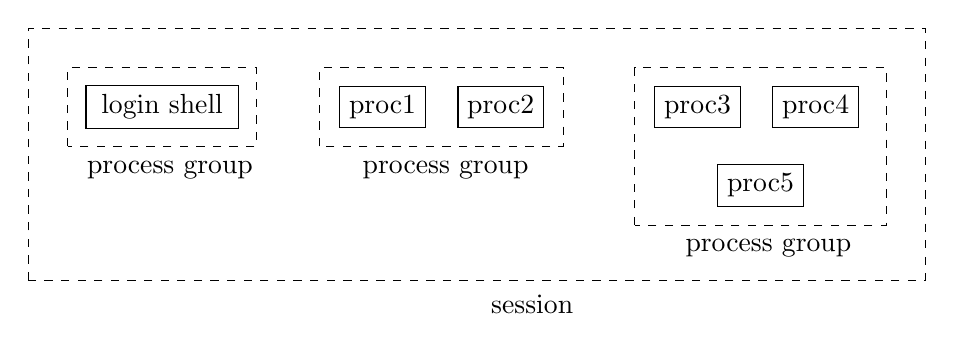
\begin{tikzpicture}
\uncover<1-> { \node [rectangle, minimum height=1em, minimum width=5.5em,draw] at (0,0) {login shell}; }
\uncover<1-> { \draw [dashed] (-1.2, -0.5) rectangle (1.2,0.5) node [xshift=-1.1cm, yshift=-1.3cm, align=center] {process group}; }

\uncover<2-> { \node [rectangle, minimum height=1em, draw] at (2.8,0) {proc1}; }
\uncover<3-> { \node [rectangle, minimum height=1em, draw] at (4.3,0) {proc2};}
\uncover<4-> { \draw [dashed] (2, -0.5) rectangle (5.1,0.5) node [xshift=-1.5cm, yshift=-1.3cm, align=center] {process group}; }

\uncover<5-> { \node [rectangle, minimum height=1em, draw] at (6.8,0) {proc3}; }
\uncover<5-> { \node [rectangle, minimum height=1em, draw] at (8.3,0) {proc4}; }
\uncover<5-> { \node [rectangle, minimum height=1em, draw] at (7.6,-1) {proc5}; }
\uncover<5-> { \draw [dashed] (6, -1.5) rectangle (9.2,0.5) node [xshift=-1.5cm, yshift=-2.3cm, align=center] {process group}; }

\uncover<6-> { \draw [dashed] (-1.7,-2.2) rectangle (9.7,1) node [xshift=-5cm, yshift=-3.5cm] {session}; }
\end{tikzpicture}

\visible <6-> {Session is a collection of one or more process groups }

\end{frame}

\begin{frame}[fragile,t]
  \frametitle{Sessions cont'd}

A process establishes a new session by calling the \texttt{setsid} function
\begin{codedef}
#include <unistd.h>
pid_t setsid(void);
// Returns: process group ID if OK, −1 on error    
\end{codedef}

If the calling process is not a process group leader, this fuction creates a new session. Three things happen
\begin{enumerate}
\item <2-> process becomes the \textit{session leader}, and is only process in this new session
\item <3-> the process becomes the process group leader (\texttt{pgid} ==\texttt{pid})
  \begin{itemize}
  \item if the caller is already a process group leader, then returns an error
  \end{itemize}
\item <4-> No contorlling terminal
\end{enumerate}

\end{frame}


\begin{frame}[fragile,t]
  \frametitle{Sessions cont'd}
\texttt{getsid} function returns the process group ID of a process's session leader

\begin{codedef}
#include <unistd.h> 
pid_t getsid(pid_t pid);
// Returns: session leader’s process group ID if OK, −1 on error  
\end{codedef}

if \texttt{pid} == 0, it returns the \texttt{pgid} of calling process's session leader
\end{frame}



\section{Controlling Terminal and Job Controls}

\begin{frame}[t]
  \frametitle{Controlling terminal}
\begin{itemize}
\item Session can have a single controlling terminal
\item session leader that connects to controlling terminal is \textit{controlling process}
\item process groups are divided into a single \textit{forground process group} and one or more \textit{background process groups}
\item interrupt signals are sent to foreground process group
\end{itemize}
\end{frame}





\begin{frame}[t]
  \frametitle{Controlling Terminal}
\begin{tikzpicture}
\node [rectangle, minimum height=1em, minimum width=5.5em,draw] at (0,0) {login shell};
\draw [dashed] (-1.2, -0.5) rectangle (1.2,0.5) node [midway, align=center, text width=10em, yshift=-3em] {\footnotesize background process group, session leader = controlling process};

\node [rectangle, minimum height=1em, draw] at (2.8,0) {proc1}; 
\node [rectangle, minimum height=1em, draw] at (4.3,0) {proc2};
\draw [dashed] (2, -0.5) rectangle (5.1,0.5) node [midway, align=center, text width=7em, yshift=-2.5em] { \footnotesize background process group};

\node [rectangle, minimum height=1em, draw] at (6.8,0) {proc3}; 
\node [rectangle, minimum height=1em, draw] at (8.3,0) {proc4}; 
\node [rectangle, minimum height=1em, draw] at (7.6,-1) {proc5}; 
\draw [dashed] (6, -1.5) rectangle (9.2,0.5) node [midway, align=center, yshift=-3em] {\footnotesize foreground process group};

\draw [dashed] (-1.7,-2.2) rectangle (9.7,1) node [xshift=-6cm, yshift=0.5em] {session}; 


\node [text width= 4em, align=center, circle, draw] at (2,-5.7) {\footnotesize controlling terminal};
\draw [-Stealth] (1.5,-4.7) -- (0,-1.8) node [rotate=-65, midway,align=right,text width=8em] {\footnotesize modem disconnect (hang-up signal)};
\draw [-Stealth] (2.8,-5) -- (7,-2) node [rotate=36, midway,align=left,text width=12em] {\footnotesize terminal input and terminal generated signals};
\end{tikzpicture}

\end{frame}



\begin{frame}[fragile]
  \frametitle{Job Control}

We can start a job in either the forground or the background

\begin{description}
\item[foreground] \texttt{vi main.c} starts a job in the foreground
\item[background] \texttt{make all \&} start a job in the background
\end{description}

\begin{verbatim}
$ make all > Make.out & 
[1] 1475
$ pr *.c | lpr &
[2] 1490
$              just press RETURN
[2] +  Done    pr *.c | lpr &
[1] +  Done    make all > Make.out &
\end{verbatim}

\end{frame}

\begin{frame}[t]
  \frametitle{Job Control cont'd}
The foreground jobs are affected by some special characters, which generate signals
\begin{itemize}
\item Interrupt character (typically DELETE or Control-C) generates SIGINT
\item Quit character (typically Control-bashslash) generates SIGQUIT
\item Suspend character (typically Control-Z) generatea SIGTSTP
\end{itemize}
\end{frame}


\begin{frame}[fragile,t]
  \frametitle{Job Control cont'd}

\begin{codedefnb}
1  $ cat > temp.foo &    
   [1] 1681
2  $                     
   [1] + Stopped (SIGTTIN)        cat > temp.foo &
3  $ fg %1               
4  cat > temp.foo        
5  hello, world          
6  ^D                   
7  $ cat temp.foo        
   hello, world
\end{codedefnb}

\begin{enumerate}
\item \footnotesize  start in background, but it’ll read from standard input
\item \footnotesize  we press RETURN
\item \footnotesize  bring job number 1 into the foreground
\item \footnotesize  the shell tells us which job is now in the foreground
\item \footnotesize  enter one line
\item \footnotesize  type the end-of-file character
\item \footnotesize  check that the one line was put into the file
\end{enumerate}

\end{frame}


%---------------------------------------------------------
\section{Last Words}

\begin{frame}[t]
  \frametitle{Last Words}
\begin{itemize}
\item Read chapter 10
\end{itemize}
\end{frame}

\end{document}
